\chapter{Logbook}

\begin{quote}
\textit{"This report, by its very length, defends itself against the risk of being read."} - Winston Churchill
\end{quote}

\section{Week 1}

\subsection{30/09/13 - Exploring simple case with PAM modulation}

I received the \emph{PAM.pdf} file outlining the case where a signal is
sent through a channel with AWGN and received with a timing error at the
receiver. I read through the file several times to get an understanding
of the underlying equations.

Leaving the Gram-Charlier series aside for the moment, I started getting
to grips with Mathematica and implementing the transmission system
model:

\[
X = \omega_0 g_0 + \sum_{k=1}^{40} ( \omega_{-k} g_{k} + \omega_k g_k ) + \nu
\]

where $g_k = g((\Delta + k)T)$,
$g(t) = (u_T \ast h_l \ast u_R)(t) \times cos(\theta)$ and $\nu$ is a
zero-mean Gaussian random variate with
$\sigma_{\nu}^2 = N_0 \varepsilon_R$.

I learnt the basics of the interface, and began implementing the filter
and channel impulse responses (I.R.). I need to double-check the
definition of the Root-Raised Cosine (RRC) Filter, as the impulse
response wasn't as expected.

Later, I found the correct form for the RRC \cite{[12]} and double-checked it using Octave. The equation used is listed below. A plot showed that this equation is invalid at
$t = \left [ - \frac{T_s}{ 4 \beta } , 0 , \frac{T_s}{ 4 \beta } \right ]$,
so I plan to find its limit at these points using Mathematica to obtain
the complete solution.

\[
h_{RRC}(t) = \frac{2 \beta}{\pi \sqrt{T_s}} \frac{cos \left [ (1 + \beta) \frac{\pi t}{T_s} \right ] + \dfrac{sin \left [ (1 - \beta) \frac{\pi t}{T_s} \right ]}{\frac{4 \beta t}{T_s}}}{1 - \left ( \frac{4 \beta t}{T_s} \right )^2}
\]

\subsection{01/10/13 - Implementing Raised Cosine functions}

I implemented the function above in Mathematica, and using the
\texttt{Limit} function found the value of the function at the following
undetermined points:

\[
h_{RRC}(t) = \left\{
  \begin{array}{l l}
    \dfrac{4 \beta + \pi (1 - \beta)}{2 \pi \sqrt{T_s}} & t = 0 \\
    \dfrac{\beta}{2 \pi \sqrt{T_s}} \left ( \pi sin \left [ \frac{(1 + \beta) \pi}{4 \beta} \right ] - 2 cos \left [ \frac{(1 + \beta) \pi}{4 \beta} \right ] \right ) & t = \pm \frac{T_s}{ 4 \beta } \\
    \dfrac{2 \beta}{\pi \sqrt{T_s}} \dfrac{cos \left [ (1 + \beta) \frac{\pi t}{T_s} \right ] + \dfrac{sin \left [ (1 - \beta) \frac{\pi t}{T_s} \right ]}{\frac{4 \beta t}{T_s}}}{1 - \left ( \frac{4 \beta t}{T_s} \right )^2} & \text{otherwise}
  \end{array}\right.
\]

I also implemented the Raised Cosine function for the channel function,
using the impulse response below\footnote{Proakis, ``Digital
  Communications''}. I was unable however to convolve the receiver and
transmitter filter functions using the \texttt{Convolve} function, even
when I limited the impulse response using a \texttt{UnitBox}.

\[
h_{RC}(t) = \frac{sinc \left ( \frac{\pi t}{T} \right ) cos \left ( \beta \frac{\pi t}{T} \right )}{1 - \left ( 2 \beta \frac{t}{T} \right )^2}
\]

I looked into Mathematica's treatment of the Gaussian distribution, and
figured out how to generate random noise vectors following a Gaussian
distribution, as well as how to generate a list of random binary
symbols.

After discussing the convolution issue with David Murphy, he suggested that the
channel should be initially modelled as ideal and therefore the overall
channel and filter I.R. $g(t)$ can be defined as a Raised Cosine
function, as defined above. I should therefore be ready to implement the
simple ISI model tomorrow.

\subsection{02/10/13 - Wrapping Up the Initial PAM Model}

I pulled together the Raised Cosine function and random number generator
to impiment the given simplified function for the PAM receiver output,
given below. Playing around with the settings, I was able to show how
the $g_k$ function increases with the timing error. I decided to study
the Mathematica environment a little more before carrying on with any
programming.

\[
X = \omega_0 g_0 + \sum_{k=1}^{40} ( \omega_{-k} g_{-k} + \omega_k g_k ) + \nu
\]

\subsection{03/10/13 - Delving deeper into Mathematica}

I devoted some time into looking through Michael Quinlan's notebooks and
better understanding the workings of the \texttt{Table} functions and
the various plotting options. Fortunately my notebook was corrupted so I
was able to rewrite it and understand the model a bit more. I need to
figure out what variance value the noise PDF should take on, as the
noise appears to be overwhelming the timing error effects. Translating
the resulting PDF's into patterns is another question that needs some
thought.

\subsection{Week 1 Summary}

Week 1 was mostly spent becoming acquainted with Mathematica and getting
a feel for the equations underlying PAM transmissions. A simple model of
a PAM receiver was constructed.

\subsection{Goals for Week 2}

\begin{itemize}
\itemsep1pt\parskip0pt\parsep0pt
\item
  The PAM model will need to be extended to calculate the optimum
  decision region boundary from the estimated PDF.
\item
  A better setup will be required to perform large-scale simulations
  within an acceptable time period. We will look into applying for an
  account on the Boole cluster.
\end{itemize}

\section{Week 2}

\subsection{07/10/13 - Matrix manipulations}

I decided to spend another day learning about the Mathematica
environment, in particular matrix manipulation and generation. I looked
into the \texttt{Apply}, \texttt{Map} and \texttt{Partition} functions
and wrote some examples to figure out how to convert mathematical
problems to Mathematica notation using matrices. I hope to convert the
code to use matrices tomorrow to hopefully simplify and speed things up.

I also implemented PhD student David Murphy's equation for properly calculating the AWGN
function variance from SNR\footnote{$\sigma_r^2 = \frac{L^2 - 1}{6 log_2(L) \left ( \dfrac{E_b}{N_0} \right )}$}, from last Friday's meeting.

\subsection{08/10/13 - Fixed I.R. and Kernel Density Estimation}

The first job was to rewrite the code to make use of the simple dot
operator to calculate all the ISI components\footnote{The ISI components
  are now calculated using: \[
  \left [
    \sum_{k=0}^{k=40} \left ( g_k \omega_k^j + g_{-k} \omega_{-k}^j \right ) \cdots
  \right ]^{j=\{1..m\}} = \\
\left [ 
    g_{-40} \cdots g_{-1} g_{1} \cdots g_{40}
  \right ] \bullet \left [
    \begin{matrix}
  \omega_{-40}^j  \\
  \vdots          \\
  \omega_{-1}^j   \\
  \omega_{1}^j     \\
  \vdots            \\
  \omega_{40}^j    \\
    \end{matrix}
  \right ]^{j=\{1..m\}}
  \] where $\omega_{k}^j$ is the $k$'th ISI with the $j$'th timing
  offset.}. With the new code I was able to carry out many more runs and
get much more detailed output. In addition, when I was rewriting the
code I noticed a typo in the Raised Cosine I.R. that was degrading
performance in the perfectly synchronised case. With both of these
changes made, I decided to use Kernel Density Estimation to see what
effects the timing offset has.

Using offsets of 10\textsuperscript{-15}, 0.05, 0.1 \& 0.15, the
following values of $g_k, k \in \{ -40 \dots -1, 1 \dots 40 \}$ were
calculated.

\begin{figure}[htbp]
\centering
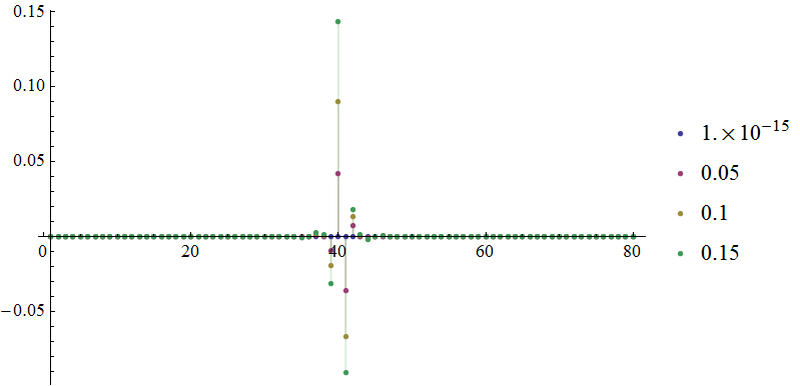
\includegraphics[width=\linewidth]{../../../plots/fyp1_w1_gklin.png}
\caption{$g_k$ linear plot}
\end{figure}

\begin{figure}[htbp]
\centering
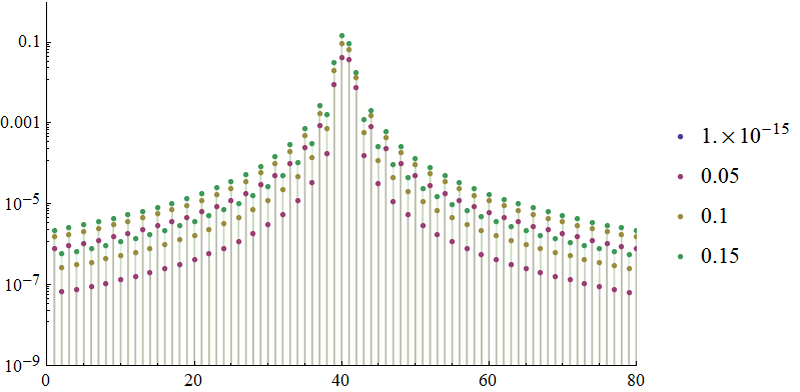
\includegraphics[width=\linewidth]{../../../plots/fyp1_w1_gklog.png}
\caption{$g_k$ log plot}
\end{figure}

Using \texttt{SmoothKernelDistribution} to perform Kernel Density
Estimation with 1 million points produced the following estimated PDFs
for both possible transmitted values. As the timing error increases, we
note that the PDF spreads out, but the mean remains steady.

\begin{figure}[htbp]
\centering
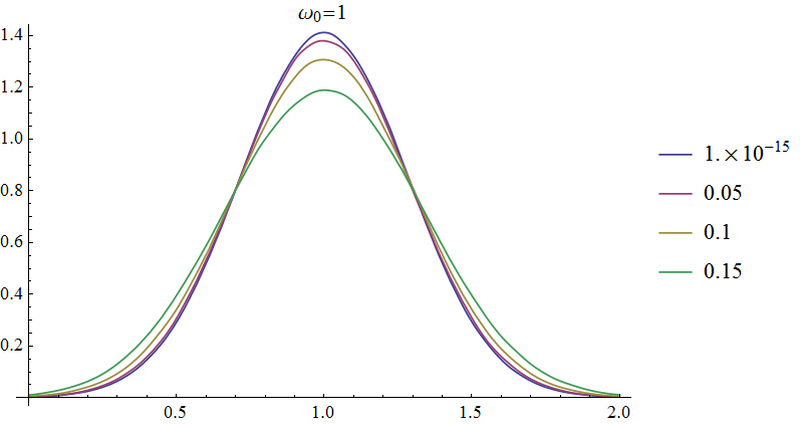
\includegraphics[width=\linewidth]{../../../plots/fyp1_w1_kde.png}
\caption{Kernel density estimation $\omega_0=1$}
\end{figure}

\begin{figure}[htbp]
\centering
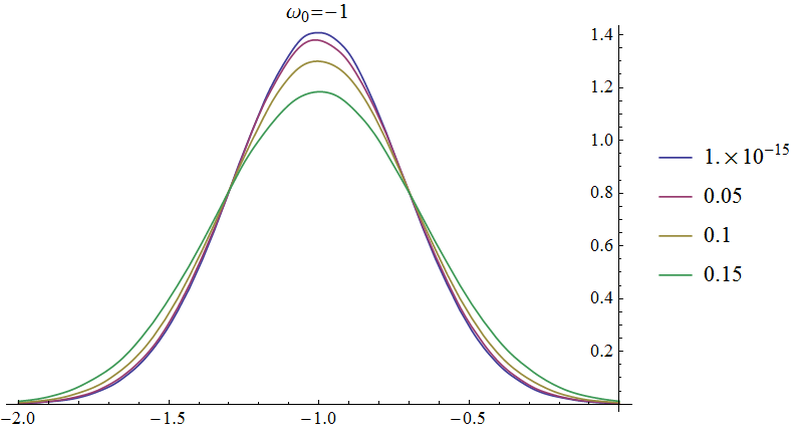
\includegraphics[width=\linewidth]{../../../plots/fyp1_w0_kde.png}
\caption{Kernel density estimation $\omega_0=-1$}
\end{figure}

\subsection{09/10/13 - Setting up Digital Comms Lab PC}

With Ger Houten's help, I set up an account on \texttt{Digital Comms Lab 1} \&
\texttt{Digital Comms Lab 2} and got the internet working. Mathematica 8
is installed and working on both machines, we will have to consider
whether an upgrade to Mathematica 9 would be useful or not. Git and VNC
or similar have to be installed next. A request was made to the Boole
cluster for access for this machine, however the email given
(\texttt{bcrisupport@bcri.ucc.ie}) was invalid.

\subsection{10/10/13 - Probing the Elec Eng network}

After finding out the Boole cluster was no more, I used today to examine
what hardware I had available to me. I got access from Ger to the public
\texttt{UEPC004} server, and from there I am able to access machines on
the Engineering network. I set up a \emph{Remote Desktop Protocol} link to
\texttt{Digital Comms Lab 1} through this server, allowing me to control
the machine from any location. I am also able to log remotely into EDA
lab machines, and run Mathematica 6 on those machines.\marginpar{The GUI
  does not work when using \texttt{ssh} to access the EDA Lab machines,
  but using the command \texttt{math} to start and operate Mathematica
  kernels does.} Ger Houten has been known to tweak machines in response to
personal requests, so if asked nicely he may let me use two or three of
these machines concurrently.

Given these resources, I feel there are three ways I could continue:

\begin{itemize}
\itemsep1pt\parskip0pt\parsep0pt
\item
  I could upgrade to the latest version of Mathematica on all machines,
  and set up a Mathematica cluster with \texttt{Digital Comms Lab 1} as
  the front end and the EDA Lab PCs as remote nodes. With this setup,
  all machines would act as one (as in a traditional cluster). This
  would be the easiest to use, but would require considerate work to set
  up.
\item
  I could use the \texttt{MathLink} interface to achieve a similar,
  lower-level version of the former, with the EDA Lab machines as
  independent, remote slaves and \texttt{Digital Comms Lab 1} sending
  commands to these slaves and collating the replies. This setup is
  distributed computing with a star topology, and would be easier to
  setup. The downside is that the code needs to manually divide the task
  between each of the nodes, and needs to be well designed to minimise
  network delays.
\item
  I could simply run the code in parallel on each of the machines
  available to me, dumping the results to text files, and collate the
  data at the end. This would require no setup, and code written on any
  machine would only require porting to another version of Mathematica.
  Additionally this seems like it would deal best with hiccups such as
  machines going down and it does not depend on a connection between the
  machines. The downside is there would be some overhead with collecting
  the results afterwards.
\end{itemize}

\subsection{Week 2 Summary}

I fixed the code written last week and began setting up my simulation
environment.

\subsection{Goals for Week 3}

\begin{itemize}
\itemsep1pt\parskip0pt\parsep0pt
\item
  Work out a setup that will allow me to carry out largeer-scale
  simulations.
\item
  Adapt the previous code to run in parallel and produce useful
  machine-readable output.
\end{itemize}

\section{Week 3}

\subsection{14/10/13 - Running longer scripts on the EDA machines}

Today I spent some time figuring out how to build and run scripts on the
EDA machines. I found that defining a module in a text file and copying
the Mathematica code into the module allows the code to be called with
input arguments, and writing the output to a text file and placing the
module in a loop allows each pass to be recorded for later
parsing\marginpar{Using the \texttt{Get} and \texttt{Put} methods. The
  \texttt{DumpSave} method is supposed to be more efficient, but was
  added after Mathematica 6.}. After running the code overnight, this
system appears to work, and is scalable over multiple machines. The
main disadvantage is the size of these files (7.7MB per 400,000 values),
so I must either figure out how to transfer them over the network or see
whether reducing the precision of the output values will reduce the file
sizes.

\subsection{15/10/13 - Reducing output size}

\marginpar{For the
  record, I could only use a fraction of them, as loading all 20 million
  samples crashed the machine for over an hour.}Given the 15GB of samples produced the night before was far too much to
pull off the machine, I copied 20 million of the samples and plotted
them to make sure the script had worked in practice. I then looked into how
I could reduce the size of the output produced, and decided to replace
the \texttt{SmoothKernelDistribution} function (which came in after
Mathematica 6.0 and therefore couldn't be used on the EDA machines) with
a fine-grained histogram function\marginpar{I am assuming that both the smooth kernel distribution and the histogram
  approach the true PDF as $\text{N} \! \rightarrow \! \infty$}. This
allowed me to add the probabilities generated in each sweep to those
generated before and keep the output to a handful of 1kB files. I ran
the simulation overnight to check it.

\subsection{16/10/13 - Moving onto 4-PAM}

Checking the output from the night before, I get a similar PDF plot as
with the \texttt{SmoothKernelDistribution} function. I therefore
modified the code to examine all 3 decision region boundaries in a 4-PAM
system and ran the simulation for 100 million samples per condition. The
resulting distributions shown below show increased probability of error
with timing error, as expected, but decision region boundaries in this
case remain the same.

\begin{figure}[htbp]
\centering
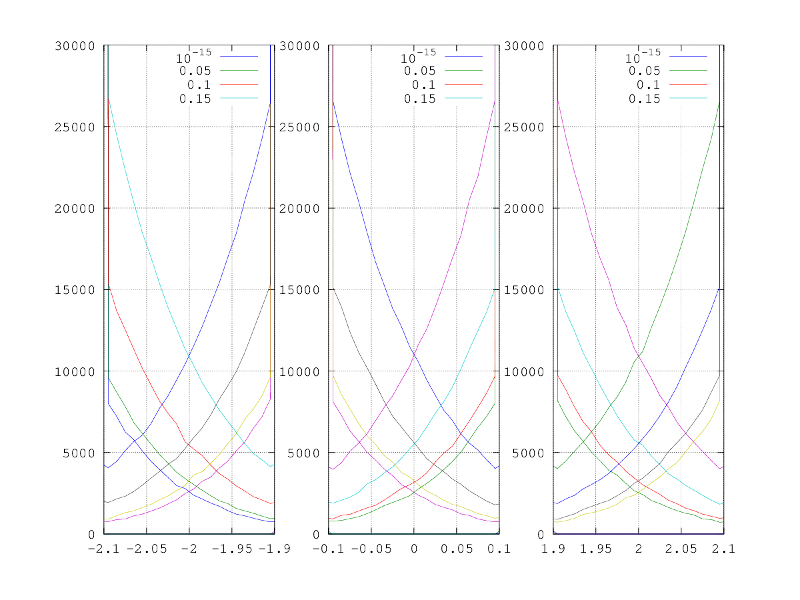
\includegraphics[width=\linewidth]{../../../plots/4pamdecision.png}
\caption[(Incorrect) non-fading received symbol PDF]{PDF for 4-PAM, $\omega_0 \in {-3,-1,1,2}$, $10^8$ samples}
\end{figure}

I could imagine finding a value for the probability of error and moving
onto PSK systems as the next steps in the process.

\subsection{Week 3 Summary}

Code was written that could be executed in parallel on multiple
machines, and this was demonstrated in practice. The code was extended
to the 4-PAM case, and showed no change in optimum decision region
boundaries. Upon later consultation with David Murphy, it seems this is because
the decision region boundaries shift due to a change in the $g_0$ term,
and not the appearance of ISI components due to the $g_k$ terms; the
latter was believed to be the expected cause, and so the $g_0$ term was
assumed to be 1 in the code.

\subsection{Goals for Week 4}

\begin{itemize}
\itemsep1pt\parskip0pt\parsep0pt
\item
  Re-run the simulations to see if implementing the change in $g_0$ with
  timing error changes the location of the optimum decision region
  boundaries.
\item
  If so, it would be interesting to see if the Gram-Charlier
  approximation produces the same boundary locations.
\end{itemize}

\section{Week 4}

\subsection{21/10/13 - Implementing the Gram-Charlier series}

Over the weekend, I implemented the $g_0$ term fix discussed in our
Friday weekly meeting and re-ran the simulation, this time across two
machines. Results showed that the Decision Region Boundary is displaced
towards the origin as the timing offset increases.

\begin{figure}[htbp]
\centering
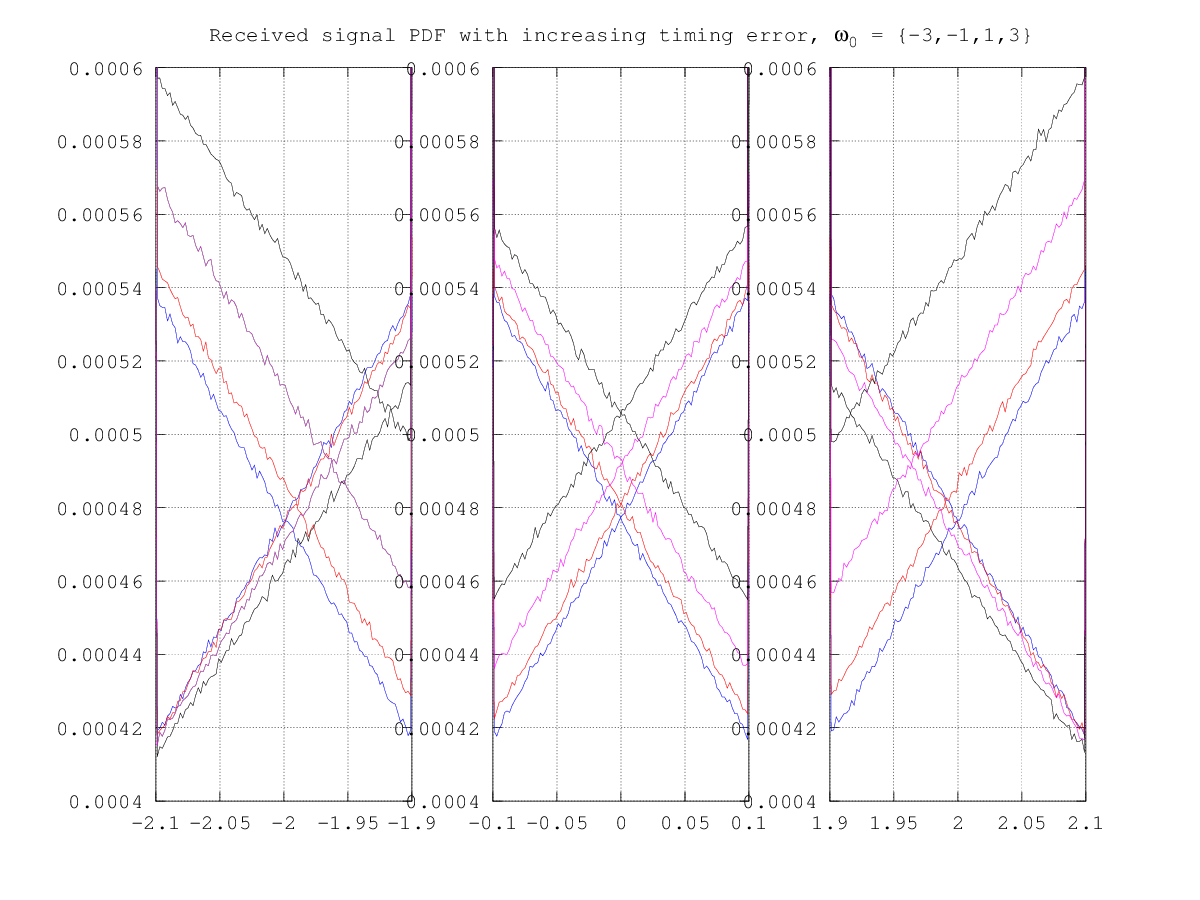
\includegraphics[width=\linewidth]{../../../plots/4pamdecisionerror.png}
\caption[Non-fading received symbol PDF]{PDF for 4-PAM, $\omega_0 \in {-3,-1,1,2}$}
\end{figure}

I spent Monday carrying out two tasks:

\begin{enumerate}
\def\labelenumi{\arabic{enumi}.}
\itemsep1pt\parskip0pt\parsep0pt
\item
  I re-wrote David Murphy's Gram-Charlier equations for Mathematica, and should be ready to try
  them out tomorrow.
\item
  I modified the PAM simulation with a coarser-grained histogram, but
  more timing offset values, in order to see how the decision variate
  varies with timing offset. The results should be available in the
  morning.
\end{enumerate}

\subsection{22/10/13 - More Gram-Charlier series}

The simulation results showed that the decision region boundaries did
decrease with timing error, however the histogram was not fine-grained
enough to accurately determine the exact boundary locations, so the
simulation was re-run with more bins.

I fixed some bugs in my implementation of the Gram-Charlier series and
was able to generate a few plots, which were very similar to those
generated by the simulator, albeit with half the amplitude. A goal for
tomorrow is to generate the plots with identical timing offsets to the
simulation and compare both plots.

\subsection{23/10/13 - Proper Gram-Charlier plots}

The simulation results had been appended to the previous set of results
by accident, so the whole thing had to be run again for tomorrow. On a
more positive note, I noticed a missing power in my implementation of
the Gram-Charlier series, and the plots are now a lot closer to those
generated previously.

\subsection{Week 4 Summary}

I implemented the Gram-Charlier series and was able to compare the
results from the simulations to the Gram-Charlier series. These are
close, but not exact, so we will have to look closely at where the
differences may be coming from.

\subsection{Goals for Week 5}

\begin{itemize}
\itemsep1pt\parskip0pt\parsep0pt
\item
  I will make use of the long weekend to run some extra-long simulations
  and compare these to the Gram-Charlier series.
\end{itemize}

\section{Week 5}

\subsection{29/10/13 - Comparing Gram-Charlier to Simulation}

The simulations ended, and I was able to compare simulated and
Gram-Charlier PDF plots. I extracted a rough estimate of the decision
region boundaries given by both methods and compared them to the
corresponding values of $2 g(\Delta)$, and found very close correlation.

\begin{figure}[htbp]
\centering
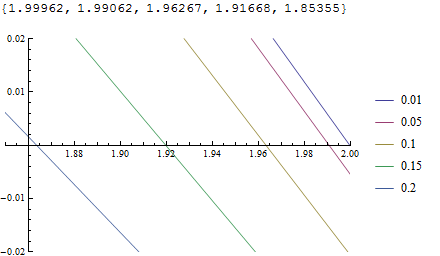
\includegraphics[width=\linewidth]{../../../plots/gcdrb.png}
\caption{Gram Charlier approximation of
$P(\omega_0=1,R)-P(\omega_0=3,R)$}
\end{figure}

\begin{figure}[htbp]
\centering
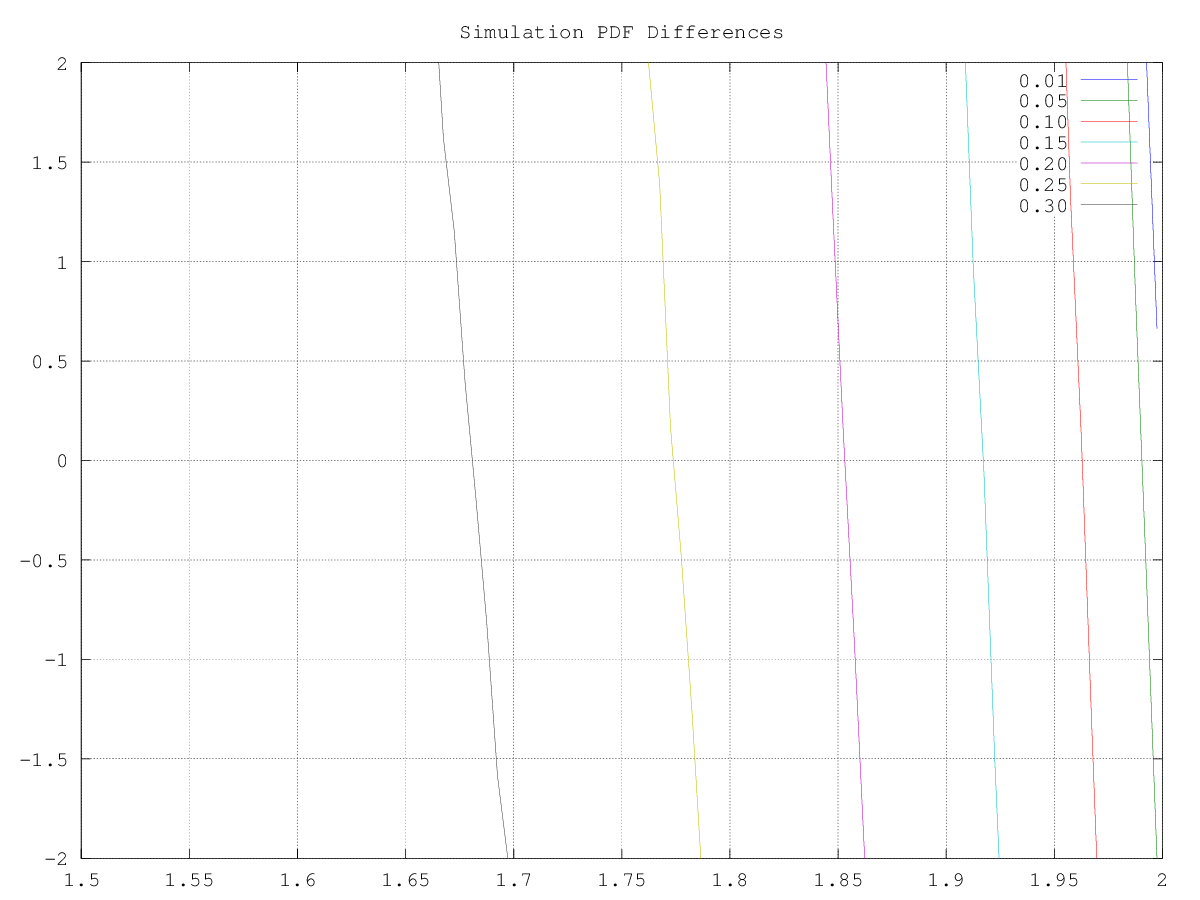
\includegraphics[width=\linewidth]{../../../plots/simdrb.png}
\caption{Simulation of $P(\omega_0=1,R)-P(\omega_0=3,R)$,
N=$3 \times 10^6$}
\end{figure}

\begin{figure}[htbp]
\centering
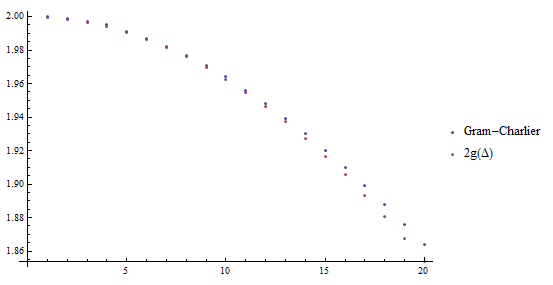
\includegraphics[width=\linewidth]{../../../plots/gc_vs_2g.png}
\caption{Comparison of Gram-Charlier Decision Region Boundaries and
$2 g(\Delta)$ estimation ($0.01 \ge \Delta \ge 0.2$)}
\end{figure}

\subsection{30/10/13 - Applying the Tikhonov Distribution}

I was able to implement the Tikhonov Distribution using the equation
provided in \emph{PAMTikhonov.pdf}:

\[
F_{\Delta} (y) = \frac{\text{Exp}\left [ \dfrac{cos(2 \pi y)}{(2 \pi \sigma_{\Delta})^2} \right ]}{I_0 \left ( \dfrac{1}{(2 \pi \sigma_{\Delta})^2} \right )} \text{  where  } -\frac{1}{2} \le y \le \frac{1}{2}
\]

Given these timing error probabilities and the optimum decision region
boundaries for each timing error, I calculated the overall optimum
decision region boundary for each timing error probability distribution
using

\[
B_{\text{OPT}} \sim \sum_{\Delta} \text{P}(\Delta) B_{\text{OPT,}\Delta}
\]

\begin{figure}[htbp]
\centering
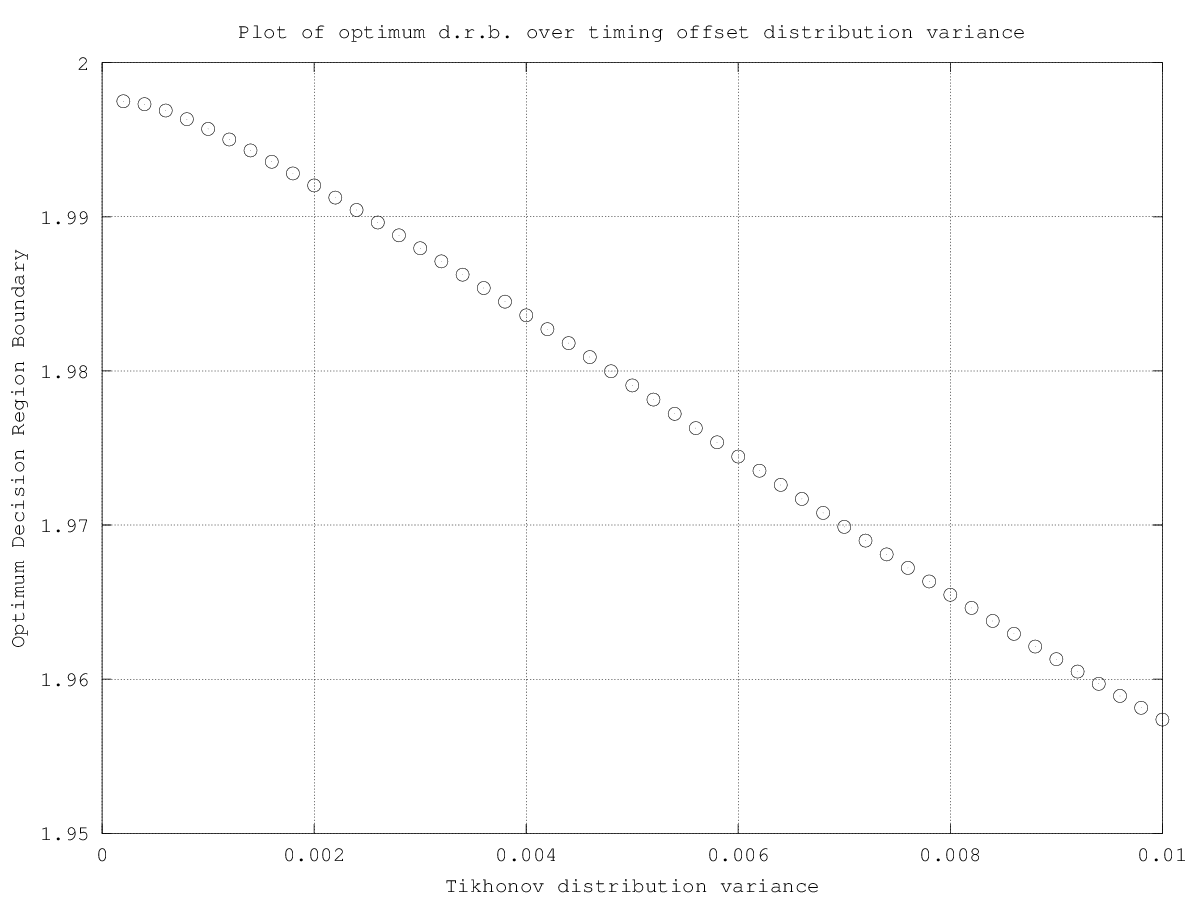
\includegraphics[width=\linewidth]{../../../plots/odrb_vs_tikhvar.png}
\caption{Optimum Decision Region Boundary for various timing error
probability distributions}
\end{figure}

It is important to note that with increasing variance, the probability
density function places more weight on larger timing errors outside the
range simulated, so these results are less accurate for higher
variances.

\subsection{Week 5 Summary}

In week 5, I calculated the optimum decision region boundary for a range
of timing offsets, through simulation and the Gram-Charlier
approximation. I demonstrated a close correlation between these
boundaries and the $2 g_k$ term. A slight difference between the
Gram-Charlier approximation was found to be due to a typo in its
implementation. I applied the Tikhonov distribution to the calculated
optimum decision region boundaries for each timing offset, in order to
calculate an optimum decision region boundary for a given Tikhonov
distribution of timing offsets

\subsection{Goals for Week 6}

\begin{itemize}
\itemsep1pt\parskip0pt\parsep0pt
\item
  On the simulation side, a key goal for week 6 is to randomly generate
  timing offsets according to the Tikhonov distribution and apply these
  to the simulation as timing offsets, in order to verify correlation
  with the Gram-Charlier and $2 g_k$ approximations.
\item
  A typo in the Gram-Charlier implementation has been found and
  corrected, and it would be interesting to see if this approximation
  matches $2 g_k$.
\end{itemize}

\section{Week 6}

\subsection{04/11/13 - Fixing errors}

David Murphy took a look at my code and spotted errors which I fixed. The fixed
Gram-Charlier implementation was found to match $2 g_k$ very closely.
The fixed simulation was left to run overnight; unfortunately
Mathematica 6.0 running on the Unix machines was unable to run it, so
the number of points had to be reduced.

\subsection{05/11/13 - Corrected simulation results}

The produced PDFs were too inaccurate to properly calculate the zero
crossing points, so the simulation will have to be run over several
days.

\subsection{Week 6 Summary}

A simulation was constructed that generated timing error offsets
according to a Tikhonov distribution of predetermined variance, and used
to produce received symbol PDFs. The simulation was found to run very
slowly, and could only be run on Mathematica 9. Ger Houten has been asked
whether it would be possible to upgrade the Unix machines to this
version and he will look into it.

\subsection{Goals for Week 7}

\begin{itemize}
\itemsep1pt\parskip0pt\parsep0pt
\item
  Continue running the simulation, trying to speed it up if at all
  possible.
\end{itemize}

\section{Week 7}

\subsection{11/11/13 - Returning to the UNIX machines}

The UNIX machines were upgraded to Mathematica 9 over the weekend, so I
was able to port the code in order to run off these. In addition, David Murphy
suggested that I look into parallelizing the code. Since these were
dual-core machines I was able to make use of Mathematica's
\texttt{ParallelTable} function to reduce run times a little. The
simulation will have to run over several days, however, as the expected
deviation in optimum decision region boundary is very small.

\subsection{19/11/13 - Day 9 of Week 7}

After several days of running the simulations, we found the optimum
decision region boundaries given by the simulations, in red, converged
to roughly those predicted by averaging the optimum decision region
boundary of a timing offset over the Tikhonov distribution of timing
offsets, in blue, given by the equation:

\[
B_{\text{OPT}} \sim \sum_{\Delta} \text{P}(\Delta) B_{\text{OPT,}\Delta}
\]

\begin{figure}[htbp]
\centering
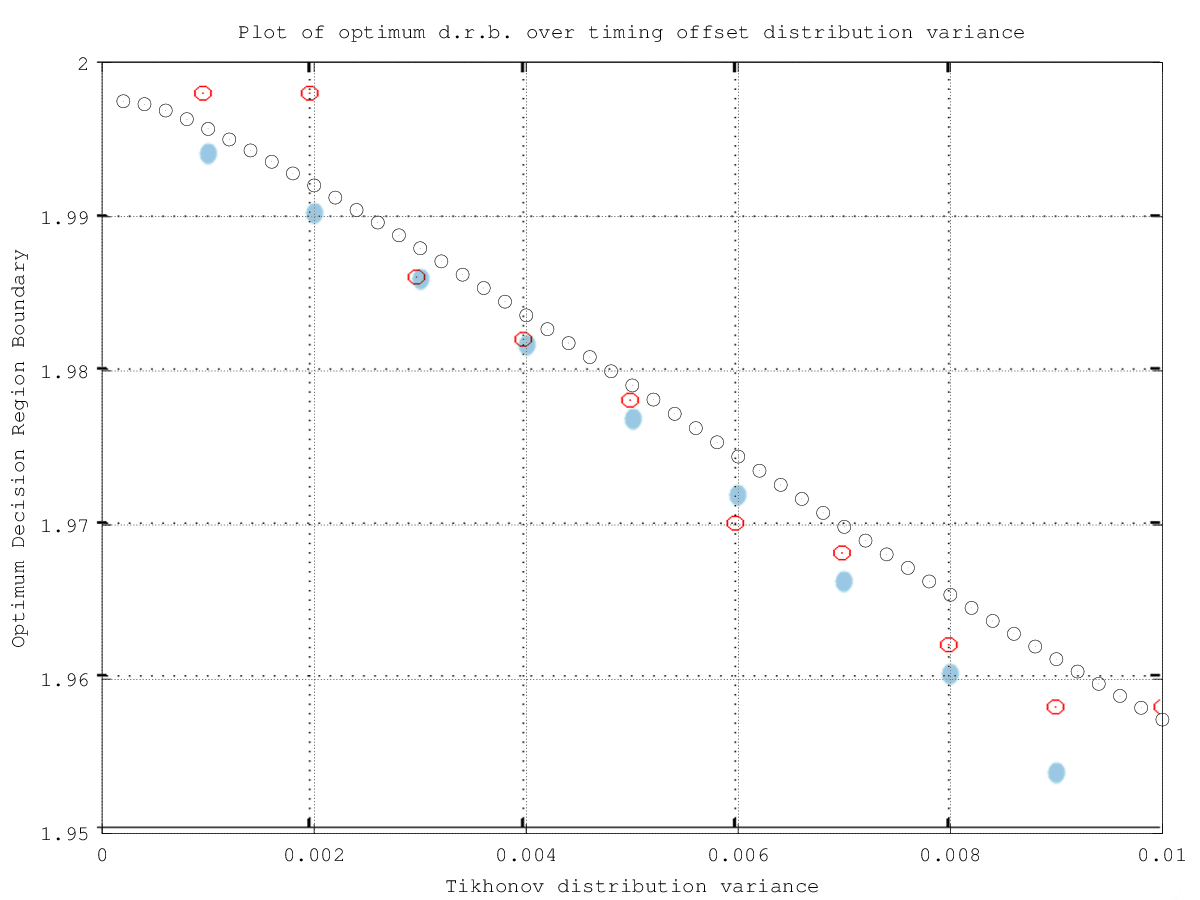
\includegraphics[width=\linewidth]{../../../plots/opt_dec_reg.png}
\caption[Optimum Decision Region Boundary for various timing error
probability distributions]{Optimum Decision Region Boundary for various timing error
probability distributions. Black: estimate found by averaging fixed timing errors over Tikhonov distribution; Blue: analytical result determined by David Murphy; Red: simulation results.}
\end{figure}

\subsection{Week 7 Summary}

Simulations supported the theory that the optimum decision region
boundary in the presence of statistically distributed receiver timing
errors will decrease from the expected value. Additionally, it was shown
through simulation that the new optimum decision region boundary can be
approximated, assuming a known distribution of these timing errors, by
averaging the optimum decision region boundary given each timing offset
over the distribution of timing offsets.

\subsection{Goals for Week 8 onwards}

\begin{itemize}
\itemsep1pt\parskip0pt\parsep0pt
\item
  Verify that the Gram-Charlier series provides an adequate
  approximation to the received symbol PDF in the presence of timing
  errors.
\item
  Provide numerical values for the probability of error $P_e$ in the
  presence of a distribution of timing errors.
\end{itemize}

\section{Week 8}

\subsection{Week 8 Summary}

After spending the Christmas break reviewing the literature on Rayleigh
fading, mainly \emph{Proakis}, I implemented the Rayleigh distribution
as a modified Nagakami-n distribution
\marginpar{The Rayleigh distribution is a special case of the Nagakami-n distribution, with n=1}
I implemented this as well as a multi-receiver combining system and
added it to the existing simulation. Following a meeting with David Murphy and
Colin Murphy, we decided to proceed as follows:

\begin{itemize}
\itemsep1pt\parskip0pt\parsep0pt
\item
  Run simulations similar to those run before Christmas to determine
  numerically the optimum decision region boundaries and corresponding
  error probabilities in the presence of Rayleigh fading with Equal Gain
  Combining (EGC).
\item
  Alongside this, attempt to provide an analytical derivation for the
  optimum decision region boundaries in the presence of timing errors in
  a non-fading environment. Should the above simulations show merit in
  modifying the decision region boundaries, this could then be adapted
  to the fading case later on.
\end{itemize}

\subsection{Goals for Week 9}

\begin{itemize}
\itemsep1pt\parskip0pt\parsep0pt
\item
  Implement the simulation. This is expected to run for the duration of
  Week 8, and demonstrate the optimum decision region boundaries for an
  EGC receiver with Rayleigh fading. The main goal is to determine if
  different decision region boundaries would reduce the probability of
  error.
\item
  Attempt to describe the system analytically, ignoring fading. This
  will be based on a Gram-Charlier approximation.
\end{itemize}

\section{Week 9}

\subsection{13/01/14 - Examining combining and fading}

Over the weekend, three separate approximate simulations were run to
examine receiver performance in three cases:

\begin{enumerate}
\def\labelenumi{\arabic{enumi}.}
\itemsep1pt\parskip0pt\parsep0pt
\item
  Similar to before Christmas, a single-receiver system in a non-fading
  environment
\item
  A multi-antenna system using EGC in a non-fading environment
\item
  An EGC system in the presence of Rayleigh fading
\end{enumerate}

Initial simulations for case 3. showed reduced optimum decision region
boundaries in the presence of Rayleigh fading, which appeared to remain
constant with changing timing offset variance. A simulation of case 2.
showed changing optimum decision region boundaries for different timing
offset variances. A more detailed simulation of case 3. examining more
variances was commenced, and is expected to finish mid-week.

\subsection{14/01/14 - Planning an analytical analysis of the non-fading
case}

I found an implementation of the Gram-Charlier series and Tikhonov
distribution I had developed previously that could be used as a basis
for an analytical exploration of the project topic. The code produces a
Gram-Charlier PDF for a range of timing offsets, calculates the optimum
decision region boundary for each, and averages these boundaries over
the Tikhonov distribution. David Murphy suggested that while this approach
wasn't mathematically correct, if the Gram-Charlier PDF's were averaged
over the Tikhonov distribution to provide an overall PDF, the optimum
decision region boundary could be calculated from this.

\subsection{15/01/14 - Evaluating the Gram-Charlier distribution over
the Tikhonov distribution}

I carried out the changes detailed above, and added a loop to
numerically estimate the location of the PDF crossings, thereby
estimating the optimum decision region boundaries. Unfortunately there
was not enough time to run the code over all possible conditions.

One of the simulations begun at the start of the week quit unexpectedly,
and had to be restarted, moving back the expected end-date for the
simulations to Friday.

\subsection{16/01/14 - Results for the above}

I was able to run the Tikhonov-Gram-Charlier code described above and
thus plot the optimum decision region boundaries for
Tikhonov-distributed timing offsets, assuming a Gram-Charlier
approximation for the received symbol. These correlated strongly with
the optimum boundaries found through simulation.

\begin{figure}[htbp]
\centering
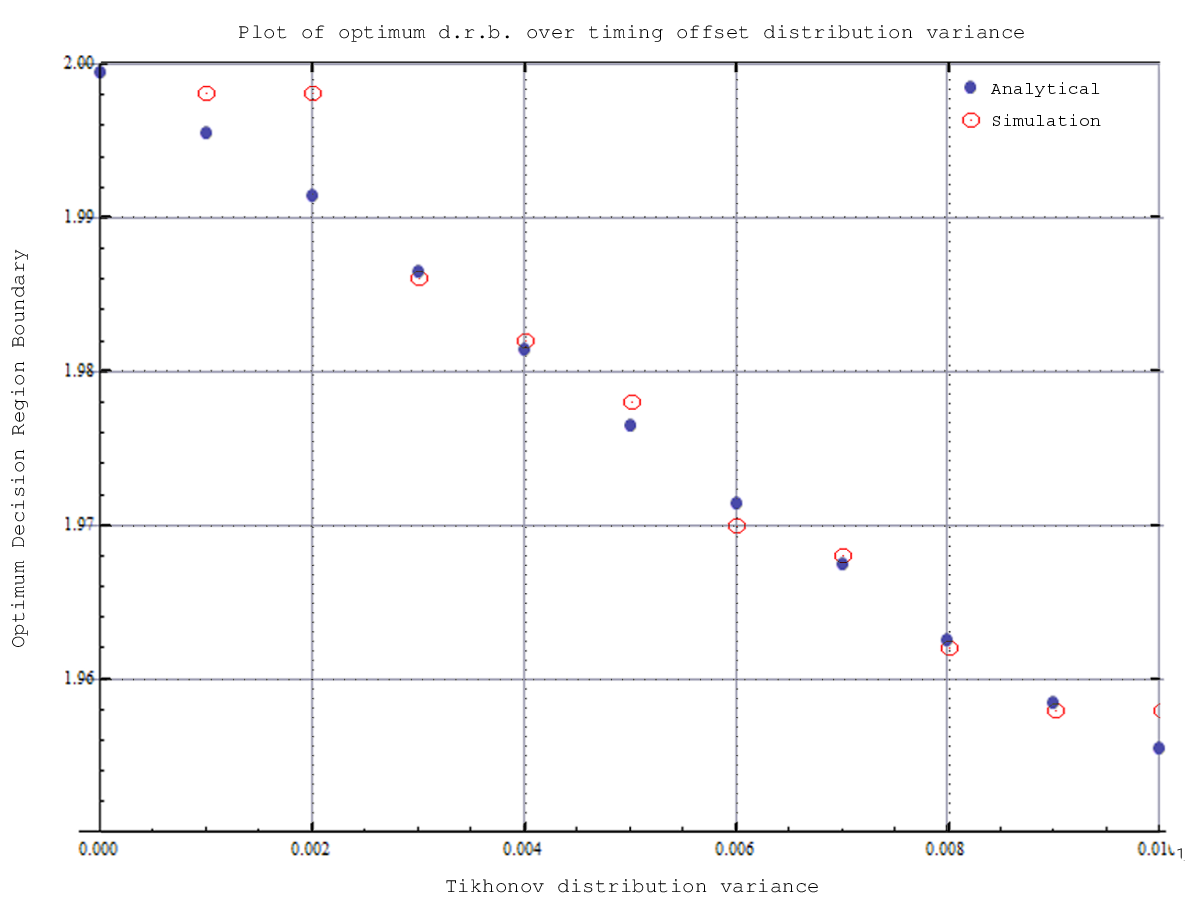
\includegraphics[width=\linewidth]{../../../plots/opt_dec_reg_analytic.png}
\caption[Optimum DRb vs. timing error variance]{Plot of optimum decision region boundaries versus
Tikhonov-distributed timing error variance, from Gram-Charlier
approximation and simulation respectively}
\end{figure}

\subsection{Week 9 Summary}

A simulation covering the 4-PAM case studied before Christmas was
extended with a 4-channel EGC system and simulated Rayleigh channel
fading. This simulation was run over the course of the week and
(\emph{proved xyz}\ldots{})

A rough analytical study of the non-fading timing error model examined
before Christmas was carried out. The PDF's of various cases with a
fixed timing offset were generated, and averaged over a discretized
Tikhonov distribution to estimate the PDF of the system in the presence
of Tikhonov distributed timing offsets. This was carried out for a range
of Tikhonov distribution variances to examine different conditions. The
optimum decision region boundary for each condition was found
numerically and found to correlate strongly with the locations
determined through simulation previously, with the exception of some
low-variance points.

\subsection{Goals for Week 10}

\begin{itemize}
\itemsep1pt\parskip0pt\parsep0pt
\item
  Examine the performance of the system in the presence of Rayleigh
  distributed channel fading.
\item
  Determine the probability of error of the system in the non-fading
  case, and evaluate any performance gains from using the calculated
  optimum decision region boundaries.
\end{itemize}

\section{Week 10}

\subsection{20/01/14 - Rayleigh Fading Results}

Simulation ended over the weekend and showed an optimum decision region
boundary around 1.72, for Tikhonov variances of 0.001 to 0.010. This is
an interesting result, as it suggests that in this particular case the
optimum decision region boundary is only loosely related to the Tikhonov
variance, which would imply that knowledge of the timing statistics is
less important in implementation than previously thought.

David Murphy produced an analytical solution for the optimum decision region
boundary in the non-fading case, which demonstrated clear BER gains
(20-33\%).

\subsection{21/01/14 - Implementing David's suggestions}

Following some consideration, Dave suggested that the SNR of 8dB used in
the simulation was too low for 4-PAM, and it's possible that the ODRB of
1.72 seen was the lower bound for the ODRB. We settled on a more
reasonable SNR of 20dB, and decided to apply each set of random
conditions to both possible sent symbols $\omega_0$ = 1,3 so that we would
only have to run the simulations once. Another suggestion made by David Murphy
was to apply a different timing offset to each channel, as each channel
has a separate receiver, and therefore independent timing. I also
implemented Maximal-Ratio Combining as an option in order to compare the
performance of both systems.

\subsection{Week 10 Summary}

This week we were able to show reduced optimum decision region
boundaries in the presence of Rayleigh fading with Equal-Gain Combining.
These results showed that the performance of the EGC receiver could be
considerably improved when facing low SNR. It was decided that the
short-term goal would be to evaluate the receiver's performance with a
more reasonable SNR, and compare it to the performance of a
Maximal-Ratio Combining system under similar conditions.

Work stopped mid-week to facilitate the author's funding application,
and is expected to resume in full next week.

\subsection{Goals for Week 11}

\begin{itemize}
\itemsep1pt\parskip0pt\parsep0pt
\item
  Evaluate the error rate of an EGC receiver with optimised decision
  region boundaries in Rayleigh fading with an SNR of 20dB.
\item
  Similarly, evaluate the error rate of a MRC receiver in similar
  conditions.
\item
  Compare and contrast the performance of each, taking into account the
  higher area and power requirements of the latter.
\end{itemize}

\section{Week 11}

\subsection{27/01/14 - Simulating EGC and MRC}

The changes discussed in the last entry were implemented, and both
simulations started.

\subsection{30/01/14 - EGC vs MRC results}

These simulations took a little longer than expected due to the extra
processing required for MRC. Error rates were found to decrease after
redefining the decision region boundary of the EGC receiver. The MRC
system suffered more from the effects of the timing error, but the
reduced EGC error rates were still a good bit higher than the equivalent
error rates using MRC. Nonetheless, a 20-33\% improvement was found over
the un-tweaked decision region boundaries.

Redefining the decision region boundary for the MRC also showed
improvements, although these were a more modest 7-20\%.

\begin{figure}[htbp]
\centering
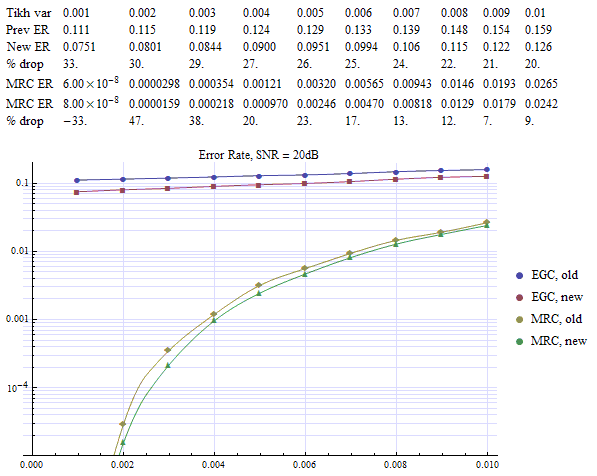
\includegraphics[width=\linewidth]{../../../plots/egc_mrc_20db.png}
\caption{EGC and MRC error rates, SNR=20dB}
\end{figure}

\subsection{01/02/14 - SNR increase to 28dB}

In order to determine how much of an effect noise has on the system in
the presence of fading, the simulation was restarted with an SNR of
28dB.

\subsection{Week 11 Summary}

The simulations ran this week proved that an error rate reduction could
be obtained by merely redefining the location of the decision region
boundaries, in the Rayleigh fading case. Although the EGC system could
not be made to perform with comparable performance to the MRC system, we
demonstrated rapidly deteriorating MRC performance with more severe
timing offsets, vindicating our study of the issue.

\subsection{Goals for Week 12}

\begin{itemize}
\itemsep1pt\parskip0pt\parsep0pt
\item
  Examine other conditions to gain a more general understanding of the
  effects of timing offsets in Rayleigh fading channels.
\item
  Start on the analytical examination of timing offset.
\item
  Compile a presentation for the seminars.
\end{itemize}

\section{Week 12}

\subsection{03/02/14 - Presentation work}

The results from the 28dB run showed very similar error rates,
confirming my suspicion that the effects of fading are dominating over
the effects due to AWGN seen in the non-fading case. A simulation at
12dB was started to see if this remained true at lower SNR's.

\begin{figure}[htbp]
\centering
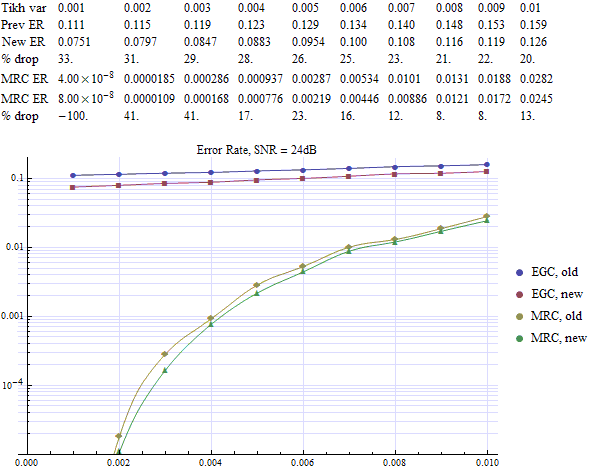
\includegraphics[width=\linewidth]{../../../plots/egc_mrc_28db.png}
\caption{EGC and MRC error rates, SNR=28dB}
\end{figure}

The seminar presentation was also compiled.

\subsection{06/02/14 - Presentation test run and rework}

The presentation was given a test-run, leading to improvements in the
clarity of the descriptions.

The simulation ended, but unfortunately it turned out that the EGC
simulation had been ran with an SNR of 8dB, so had to be run again.

David Murphy announced he has been able to start the analytical proof of the
timing offset, and we should be able to hear from him at the start of
next week. I am planning on using his code as a base to build upon for my project.

\subsection{Week 12 Summary}

A relatively quiet week, with a focus on the seminar presentation.

\section{Week 13}

\subsection{11/02/14 - Analytical description of non-fading case}

David Murphy provided a proof for the Gram-Charlier approximation of the
non-fading case, along with some accompanying code. Used the
Gauss-Legendre method to combine the Gram-Charlier solution for a fixed
timing offset with the Tikhonov timing offset distribution to provide a
solution for the PDF at the input to the receiver, which is too long to
reproduce here in full, but is approximately given by:

\[
\dfrac{b-a}{2} \sum\limits_{i=1}^N \omega_i \: T \left (\dfrac{b-a}{2} z_i - \dfrac{b+1}{2} \right ) \: GC \left (\dfrac{b-a}{2} z_i - \dfrac{b+1}{2} \right )
\]

where $\omega_i = \dfrac{2}{(1-z_i)(P(z_i))^2}$ and $z_i$ are the roots
of the Legendre polynomial $P_n(z)$.

I spent some time examining the Mathematica code he used to examine the
above, and decided as an introduction to try to extend it to the
Equal-Gain comining case. I used the property that for the PDF of the
sum of two independent variants is the convolution of each variant's PDF
(ie. for two variants $X_1$ and $X_2$ with PDF $f_1(x)$ and $f_2(x)$,
the PDF of $Y=X_1+X_2$ is $f_Y(x) = f_1(x) \ast f_2(x)$) to express the
PDF of an m+1 antenna EGC system as

\[
f_{EGC}(x) = f^{m \ast}(x)
\]

where $f(x)$ is the PDF at each antenna and $f^{2 \ast}(x)$, for
example, is the double convolution $f(x) \ast f(x) \ast f(x)$).

I was then able to use the Gauss-Legendre method to describe this as an
m-fold sum:

\[
\begin{matrix*}[l]
f_{EGC}(y) = f^{m \ast}(y) \simeq \sum\limits_{a_1=1}^{n_f} \cdots \sum\limits_{a_m=1}^{n_f} \: 3^m \omega_{a_1}  \cdots \omega_{a_m} \times \\
f(3 z_{a_m} - 3 z_{a_{m-1}}) \cdots f(3 z_{a_2} - 3 z_{a_1}) \: f(3 z_{a_1} + 2) \: f(y - 3 z_{a_m} - 2) 
\end{matrix*}
\]

I was unfortunately unable to test this code before end of day.

\subsection{12/02/14 - Viability of independent variate route}

During an email conversation with David Murphy, he suggested that the
convolution route might be difficult to implement in terms of processing
requirements, and suggested instead that in the case of the MRC system,
the independence of the timing error and fading statistics of each
receive channel means that a "joint" PDF describing the probability of
all timing and fading variables can be constructed by taking the product
of each timing and fading PDF. Therefore we can derive a Gram-Charlier
distribution conditioned on a particular set of timing offsets and
fading factors, calculate the BER of this theoretical system, and
average this over the distribution of timing offsets and fading factors
described by the joint PDF.

\subsection{13/04/14 - MRC adaptation of Gram-Charlier distribution}

I went over the process described yesterday in more detail with David Murphy to ensure I fully understood it,
and began to implement it by replacing all the $g_k(\Delta)$ terms in
his implementation of the non-fading Gram-Charlier series with
$\alpha_1^2 g_k(\Delta_1) + \alpha_2^2 g_k(\Delta_2)$ to reflect the
effects of fading with a 2 antenna system. In this case, the expected
(synchronized) DRB which was previously simply $2 g_0(0) = 2$ is now
given by
$2(\alpha_1^2 g_0(0) + \alpha_2^2 g_0(0)) = 2(\alpha_1^2 + \alpha_2^2)$.

Testing this model, I noticed oscillations at the tails of the
distributions which made it impossible to calculate the optimum DRBs, as
there were multiple PDF crossings.

\subsection{14/04/14 - Explaining the oscillations}

I raised the issue with David Murphy, and it turned out that I had forgotten the
effects of fading on the channel Gaussian noise. The variance of this
noise is scaled by the effects of noise, in this case by
$(\alpha_1 + \alpha_2)$. Making this correction I was able to determine
the optimum DRB to be equal to
$2(\alpha_1^2 g_0(\Delta_1) + \alpha_2^2 g_0(\Delta_2))$, as expected.

\subsection{Week 13 Summary}

In this week I examined David Murphy's derivation and modelling of the non-fading
case using the Gram-Charlier series, and make a start on my own piece of
the analytical work. I successfully extended his derivation to describe
the decoder input PDF for a 2 antenna MRC system given known fading
statistics and timing offsets, which puts me in a good position to
extend this to a more thorough analytical exploration of receiver
performance with diversity.

\subsection{Goals for Week 14}

\begin{itemize}
\itemsep1pt\parskip0pt\parsep0pt
\item
  Evaluate the BER for given fading and timing statistics.
\item
  Average the BER over fading and timing offset distributions to
  determine the average BER for a given system.
\end{itemize}

\section{Week 14}

\subsection{16/02/14 - Bit Error Rate Calculation}

I implemented the BER calculation for fixed fading and timing statistics
as two integrals over the Gram-Charlier PDF approximations, using a
given decision region boundary to bound the integrals. Using this I was
able to determine the BERs using both the sub-optimum decision region
boundaries $2(\alpha_1^2 + \alpha_2^2)$ and the optimum decision region
boundaries calculated using last week's code.

\subsection{18/02/14 - Averaging BER over Tikhonov and Rayleigh
distributions}

The code was extended to average the BER for each timing error and
channel gain over Tikhonov and Rayleigh distributions, respectively,
using Gauss-Legendre Quadrature. In this way the average BER for given
timing offset and fading statistics can be calculated. Progress was slow
as some of the previous code has to be rewritten to fit with its new
application. Gauss-Legendre Quadrature was found to be unsuited to the
Rayleigh distribution, for reasons I am not yet sure of, so a discrete
sampling of the distribution was used instead. At the end of the day the
\emph{FindRoot} method used to determine the optimum decision region
boundaries refused to converge for certain ranges of timing error and
channel gain, so more work must be done to finish it off.

\subsection{19/02/14 - Root-finding tweaks}

I noted that the \emph{FindRoot} method had difficulty converging for
both very high and very low channel gains, as the optimum decision
region boundary in these cases are much higher or lower than usual.
Since the nature of the Rayleigh distribution dictates that these
extreme gains are still likely, I used the observation that the gain can
be roughly given by $2(\alpha_1^2 + \alpha_2^2)$ for low timing error
offsets, and instructed the \emph{FindRoot} method to start the search
at this point. This improved both the speed and possibility of
converging.

The algorithm was still having difficulty converging for any significant
timing error offset, so I greatly reduced the accuracy requirements of
the root finding algorithm, under the understanding that we are dealing
with average error rates and the goal is to show the rough gain in
performance. This brought the algorithm under control, but nonetheless
some issues remained:

\begin{itemize}
\itemsep1pt\parskip0pt\parsep0pt
\item
  For very large timing error offsets, the algorithm converged to an
  unlikely value. This is unimportant, as in these cases the system has
  failed to perform any sort of detection.
\item
  The response is somewhat oscillatory. This could be due to the
  accuracy of the Gram-Charlier series, or less likely the
  \emph{FindRoot} method.
\item
  Even more complexing, the algorithm seems to fail to converge for
  certain combinations of timing error offset. At first glance it looks
  like there is a pole or zero at these points. Again, perhaps Dave
  could suggest a fix for these points.
\end{itemize}

\emph{Insert timing error 2D density plot}

\subsection{20/02/14 - Discussion of Gram-Charlier accuracy}

I discussed the issue described above with David Murphy and Dr. Colin Murphy, and David Murphy
suggested increasing that it could be a machine precision problem, and
that increasing the precision of the variables used in the Gram-Charlier
series calculation could solve the problem. Alternatively, Dr. Colin Murphy
suggested that an acceptable answer could be obtained by truncating the
sweep to remove the areas where the \emph{FindRoot} algorithm does not
converge.

\subsection{21/02/14 - Overcoming the timing error problems}

Through some exploration, the random non-convergent regions were found
to disappear at higher AWGN variances. I therefore rose the SNR to 20dB,
and found that the oscillations in the root estimates also disappeared.

\subsection{22/02/14 - Further problems for high timing offsets}

I observed that the root finding algorithm failed to converge for large
timing error offsets. Noting that it definitely converged for timing
offsets of 0.3 and below, and that timing offsets greater than this were
extremely unlikely, I decided to truncate the timing offset averaging to
$-0.3 \le \Delta \le 0.3$.

\emph{Plot of roots verses timing error}

After implementing this I discovered that the root-finding algorithm
results still became increasingly inaccurate for higher timing offsets.
This will require further investigation to determine its cause, as left
untouched it could significantly reduce the accuracy of the model.

\subsection{Week 14 Summary}

This week saw the implementation of Bit Error Rate calculations for
given fading and timing variates, and the averaging of these over the
timing and fading probability distributions was the final step in the
implementation of a mathematical model for the described MRC system and
allowed a figure for the average BER of the system to be determined.
While testing the corners of the implementation, it was found that the
analytical approximation failed at certain timing offsets at low SNR
values, but this was ignored as larger SNR values are of interest to us.
Additionally the optimum DRB finding algorithm does not converge for
higher timing error offsets, leading to the decision to ignore the
statistically unlikely larger timing offsets. More work will have to be
done on reducing the error of the algorithm at middle timing offsets,
however.

\subsection{Goals for Week 15}

\begin{itemize}
\itemsep1pt\parskip0pt\parsep0pt
\item
  Improve the accuracy of the model for large timing error offsets.
\end{itemize}

\section{Week 15}

\subsection{24/02/14 - Root-finding-defying wiggles}

I found that the source of the root-finding errors is in ``wiggles''
near the roots of the $f_1(y)=f_3(y)$ function used to find the optimum
DRB. These seem to be caused by inaccuracies in the Gram-Charlier
approximation. Increasing the numerical accuracy did not seem to have
any difference, and increasing the length of the Gram-Charlier series
only made the oscillations much worse.

\begin{figure}[htbp]
\centering
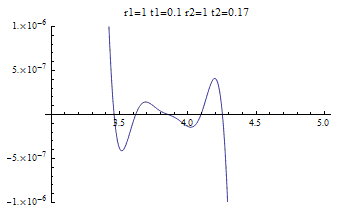
\includegraphics{../../../plots/rootfindingconfusion_M20_cropped.png}
\caption{"Wiggles" near the roots}
\end{figure}

\subsection{25/02/14 - Correct optimum DRB measurements}

A brief email exchange with David Murphy helped me understand the source of the
problem. In the model I had built, it was assumed that the instantaneous
channel gains and timing offsets were known, and used to make an
estimate of the optimum DRB, and the resulting BER was averaged over the
fading and timing error PDFs to obtain the average BER. However as
mentioned earlier, while the instantaneous channel gains are known in a
MRC system (but not an EGC system!), the timing offsets aren't. Hence,
the correct approach is to obtain an average PDF for each pair of
channel gains, deduce the optimum DRB and BER for each of those channel
gains, and then average over the fading and timing error PDFs. Therefore
the ``wiggles'' seen before will be reduced when averaging over the
Tikhonov, and shouldn't be present when the optimum DRB is calculated.

I implemented the averaging of the GC PDFs over the Tikhonov timing
offset distributions to provide an overall PDF for given channel gains
and Tikhonov variances, and from these determined the optimum decision
region boundaries. These are now used to determine the BER for different
channel gains and timing offsets, which are averaged over the Rayleigh
and Tikhonov distributions to determine the average BER.

\subsection{26/02/14 - Integration}

After a suggestion from David Murphy, I tried implementing a closed-form
solution for the integration of the Gram-Charlier PDF approximation,
given solutions for the integration of other identities. In this manner
I hoped to significantly reduce the time to determine the average BER.

Starting with the Gram-Charlier definition described earlier,

\[
f_{X\vert \Delta}(y) = \frac{1}{\sigma_X} \: \phi \! \left ( \frac{y-\mu_X}{\sigma} \right )
\]
\[
\; \; \; \; \; \; \; \; + \sum \limits_{m=2}^M \frac{\alpha_{2m}}{(2m)! \sigma_X^{2m}} \left [ \frac{1}{\sigma_X} \: \phi \! \left ( \frac{y-\mu_X}{\sigma} \right ) \: H_{2m} \! \left ( \frac{y-\mu_X}{\sigma_X} \right ) \right ]
\]

and incorporating the given identites,

\[
\int \limits_{-\infty}^x \frac{1}{\sigma} \: \phi \! \left ( \frac{y-\mu}{\sigma} \right ) dy =
\frac{1}{2} \left ( 1 + \text{erf} \! \left ( \frac{x-\mu}{\sqrt{2} \sigma} \right ) \right )
\]

\[
\int \limits_{-\infty}^x \frac{1}{\sigma} \: \phi \! \left ( \frac{y-\mu}{\sigma} \right ) H_m \! \left ( \frac{y-\mu}{\sigma} \right ) dy =
- \phi \! \left ( \frac{x-\mu}{\sigma} \right ) H_{m-1} \! \left ( \frac{x-\mu}{\sigma} \right )
\]

the solution for the integral of the Gram-Charlier series was found to
be:

\[
\int \limits_{- \infty}^x f_{X\vert \Delta}(y) = \frac{1}{2} \left ( 1 + \text{erf} \! \left ( \frac{x-\mu_X}{\sqrt{2} \sigma_X} \right ) \right )
\]
\[
\; \; \; \; \; \; \; \;  - \sum \limits_{m=2}^M \frac{\alpha_{2m}}{(2m)! \sigma_x^{2m}} \: \: \phi \! \left ( \frac{x-\mu_X}{\sigma_X} \right ) H_{2m-1} \! \left ( \frac{x-\mu_X}{\sigma_X} \right )
\]

I found that while the resulting equation approximated the result found
using numerical integration (\emph{NIntegrate}), the two did not match
exactly. An interesting question is which correct. My own gut feeling is
that the value found using \emph{NIntegrate} is correct, as the
algorithm converges to a very precise result and I have very little
confidence in my own mathematical abilities, so for the moment I will
stick with it. Then again, it is possible that numerical integration is
reflecting some unforeseen inaccuracies in my implementation of the
Gram-Charlier series, and the closed-form solutions, being
mathematically-based, are accurate.

\subsection{Week 15 Summary}

In week 15 I fixed a significant inaccuracy in the model I had built to
determine the average BER, stemming from a misconception I had acquired
from getting caught up with implementation and forgetting the top-level
picture. The numerical implementation of the analytical model seems to
be close to finished, and a few tentative tries showed poorer results
than those found through simulation. Hopefully work next week will
produce the definitive model alongside some quantitative results.

\subsection{Goals for Week 16}

\begin{itemize}
\itemsep1pt\parskip0pt\parsep0pt
\item
  Complete the implementation of the analytical model.
\item
  Try a few test runs to determine the performance of the standard and
  modified MRC system.
\end{itemize}

\section{Week 16}

\subsection{03/03/14 - Rewriting analytical implementation}

My machine turned off on Friday afternoon, and I returned from the
weekend to find that my \emph{Mathematica} notebook had been corrupted.
After some time trying to manually fix the corrupted file I decided the
task was too large and reverted to a week-old backup of the file. As
much work had been done in the time between I took the opportunity to
rewrite much of the implementation to make it clearer.

\subsection{04/03/14 - Strengthening the implementation}

Some time was spent improving the speed of execution of the
implementation and testing it at intermediate points to ensure the
results given made intuitive sense. Currently the implementation takes
roughly 25mins to run for 5 timing error and channel gain points per
channel.

\subsection{05/03/14 - Assessing the accuracy of the implementation}

I spent some more time tweaking the accuracy and precision parameters of
the \emph{FindRoot} and \emph{NIntegrate} function to reduce the speed
of execution without compromising the accuracy of the system. By looking
through the intermediate results of the implementation I found that
inaccuracies in the Gram-Charlier approximation for high timing offsets
are creating such large error rate estimations for the traditional
decision region boundaries that their reduced weighting is insufficient
to prevent their effects appearing in the averaged BER value.
Unfortunately I cannot imagine how this could be mitigated without
ignoring more than the most trivial timing offsets, which wouldn't allow
us to show off the full utility of out method.

I added memory to the Gram-Charlier distribution definition to try to
speed up the implementation a little more, and started a sweep of timing
error variances.

\section{Week 17}

\subsection{14/03/14 - Pre-open day progress}

The past weekend was spent trying to account for differences between the
analytical and simulation models. Both successfully demonstrated reduced
optimum decision region boundaries in the presence of timing errors;
however the reduction is much more severe in the simulation than using
the analytically derived results. Since I was hoping to be able to
derive the optimum DRB values analytically, this was and still remains a
major stumbling block.

David Murphy suggested a modification to the \emph{FindRoot} method which mixes
Newton's Method and the Bisection Method in order to prevent divergence,
however since this isn't currently an issue I doubt I'll have time to
implement it.

\section{Week 18}

\subsection{17/03/14 - Comparing Analytic and Simulation results
side-by-side}

I spent the weekend combining the conditional analytical and simulation
code to provide comparisons between both methods. I found that the
analytic solution grossly underestimated the spread of the received
symbol, suggesting an issue with the SNR calculations. I was able to
confirm that while the analytic method broke down somewhat at higher
timing offsets, the response remained somewhat approximate to the pdf
generated through simulation. Overall, it did demonstrate similar
characteristics to the simulation, just not to the same extent.

Suspecting that this meant that there was a simple mistake in
calculating the parameters of the Gram-Charlier approximation, I made a
simplified version and asked David Murphy to look over it.

\subsection{18/03/14 - Fixing the Gram-Charlier code}

David Murphy got back to me with two mistakes in the code:

\begin{itemize}
\itemsep1pt\parskip0pt\parsep0pt
\item
  The variable \emph{L} represents the number of symbols (4 in the case
  of 4-PAM), not the number of diversity branches as I had mistakenly
  believed.
\item
  The SNR in the case of channel fading is gained by the RMS sum of the
  channel gains ($\sqrt{\sum \alpha_i^2}$) and not the sum of the gains
  ($\sum \alpha_i$).
\end{itemize}

Implementing these changes, I saw instant improvements in the
correlation between the analytical and simulation PDFs. I also, after
some consultation with Dave, rewrote the simulation to make the timing
error on each branch independent, as he noted that while both branches
run off the same frequency generator, the clock regeneration circuits on
each branch will lead to different timing offsets, I restarted both the
standalone realistic simulation and the conditional
simulation/analytical for 2 diversity branches with the changes made to
see how closely both methods match.

\subsection{20/03/14 - A much closer match}

The comparison finished, I was able to see that the Gram-Charlier
approximation and simulation results now match very closely, even at
higher timing offset variances. To double-check that this confirms the
Gram-Charlier approximation's suitability for our purposes, I restarted
the comparison zoomed into the boundary region, as can be seen below.

\begin{figure}[htbp]
\centering
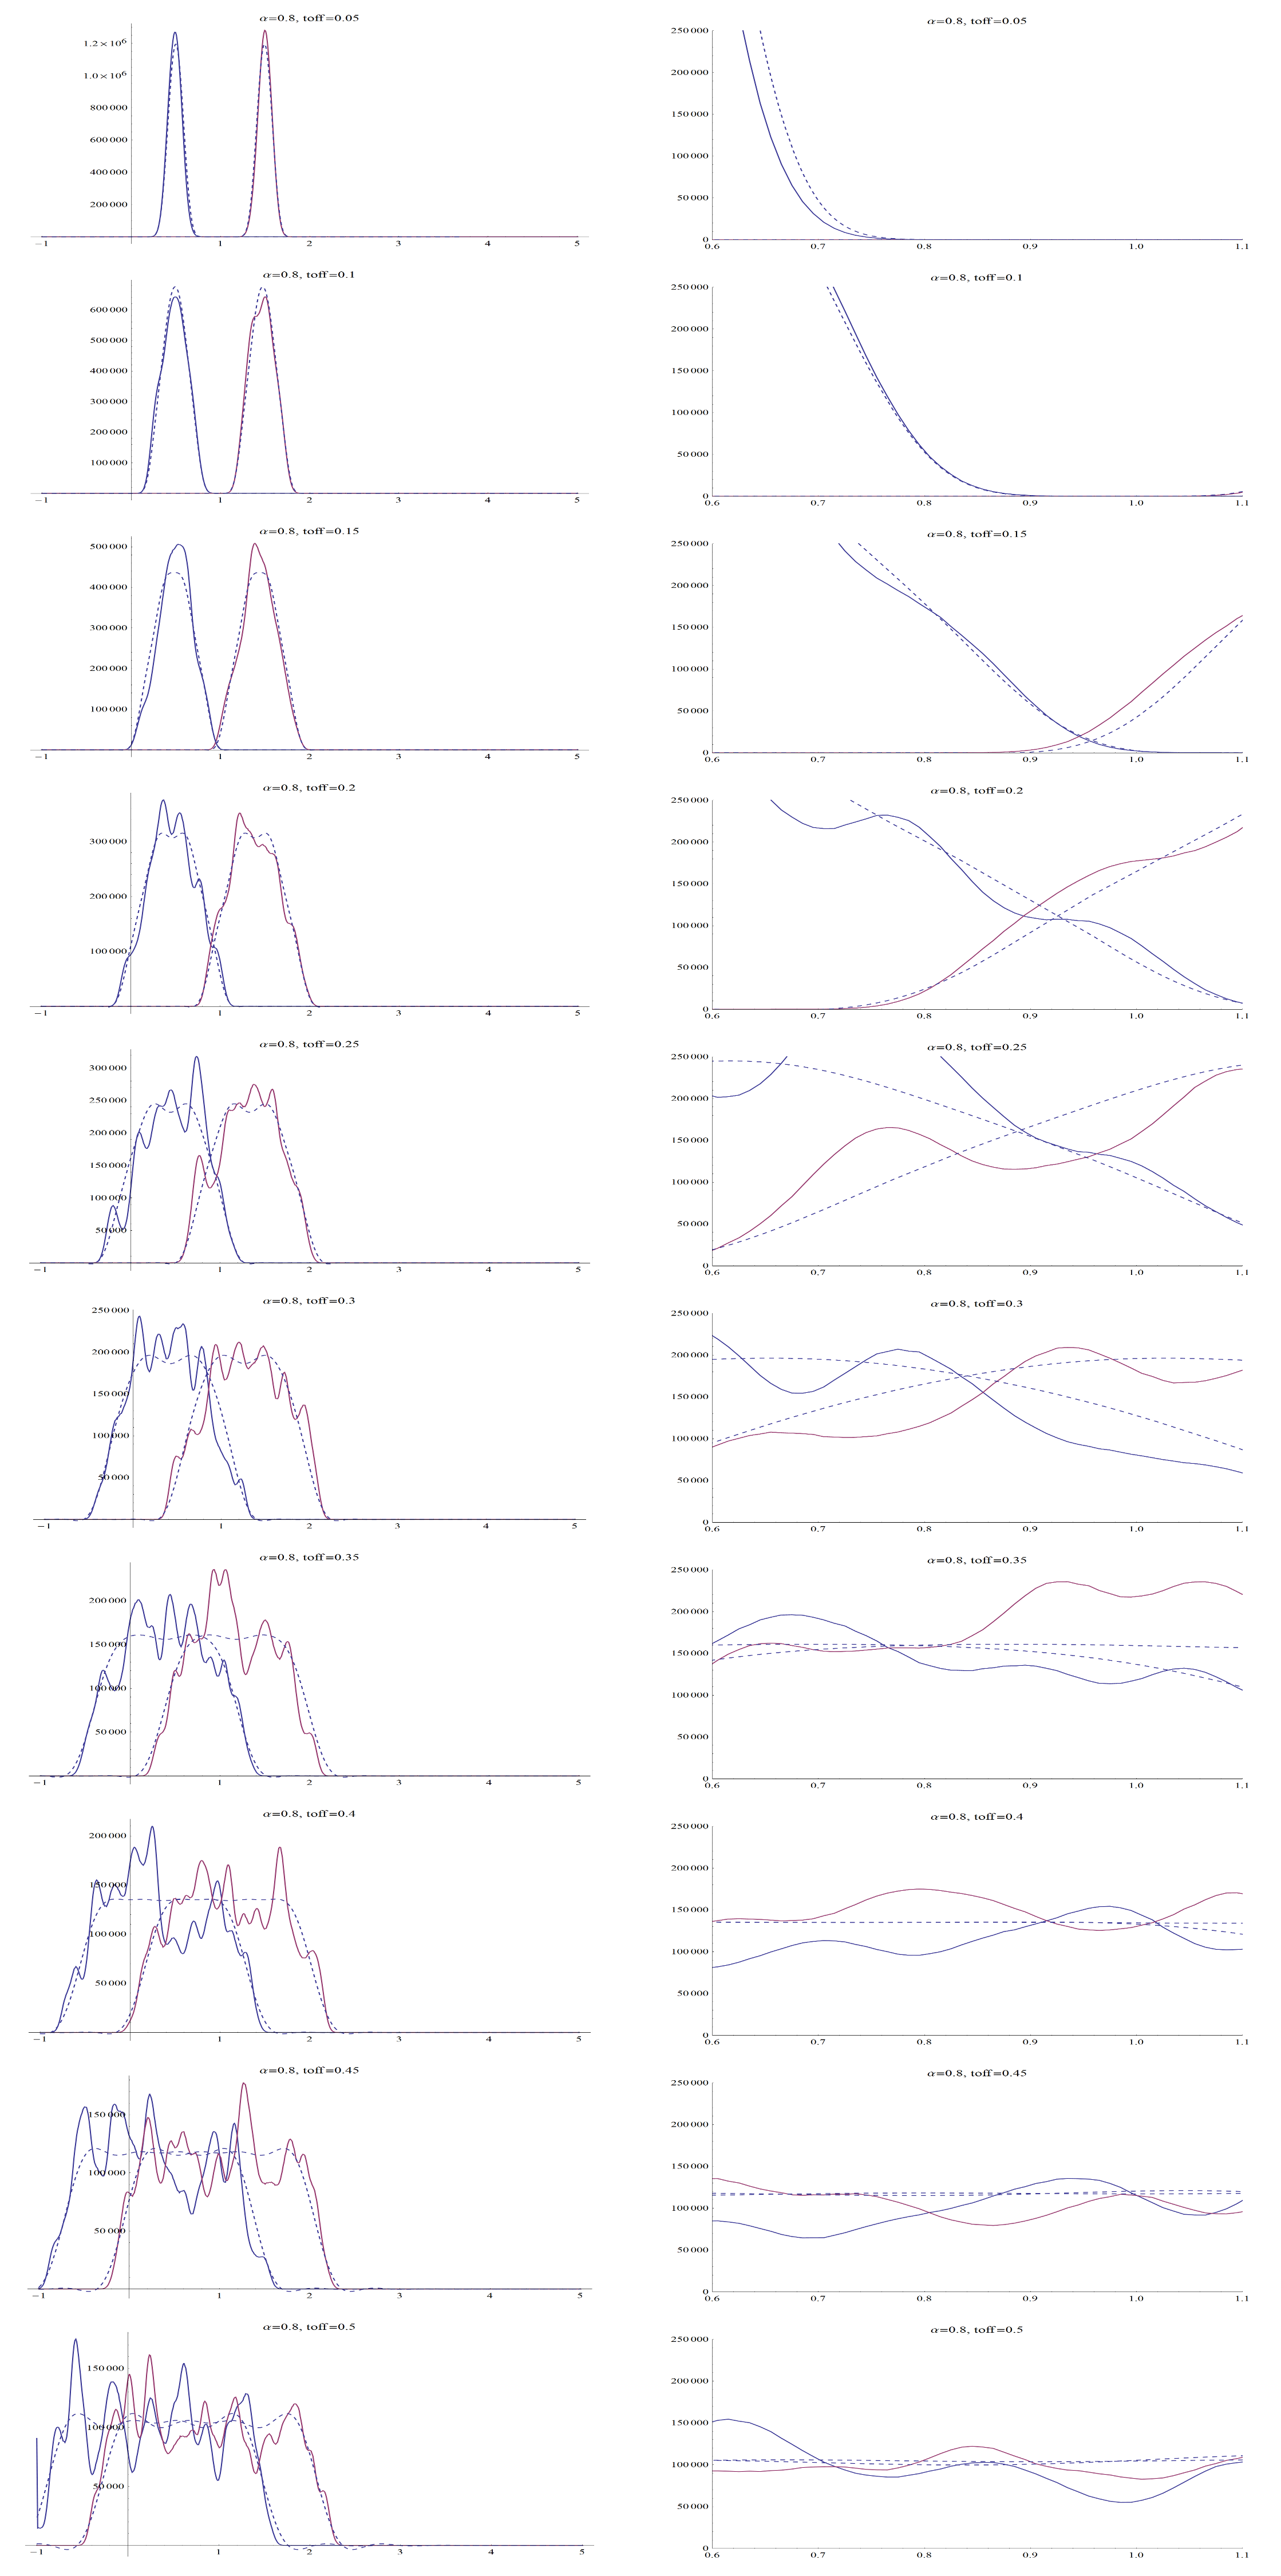
\includegraphics[height=\textheight]{comparison_scaled.png}
\caption[Simulation vs. analytical received symbol PDFs]{Sample comparison between simulation (solid) and analytic
(dashed) received symbol PDF's}
\end{figure}

\subsection{21/03/14 - A slight mistake}

The simulation ended, and I realised that I had accidentally build on the
code used to determine the results for the EGC system. Substituting the
description of the MRC system, I restarted the simulation.

\subsection{22/03/14 - Revised MRC simulation results}

The MRC simulation finished, and I was able to observe that our revised
system still gave us gains of up to 14\% in the presence of strong
timing offsets, for a 2-channel diversity system.

For added precision, I ran the simulation again. I also returned to the
analytical description to see if the optimum decision region boundaries
could be determined from the latter.

\begin{figure}[htbp]
\centering
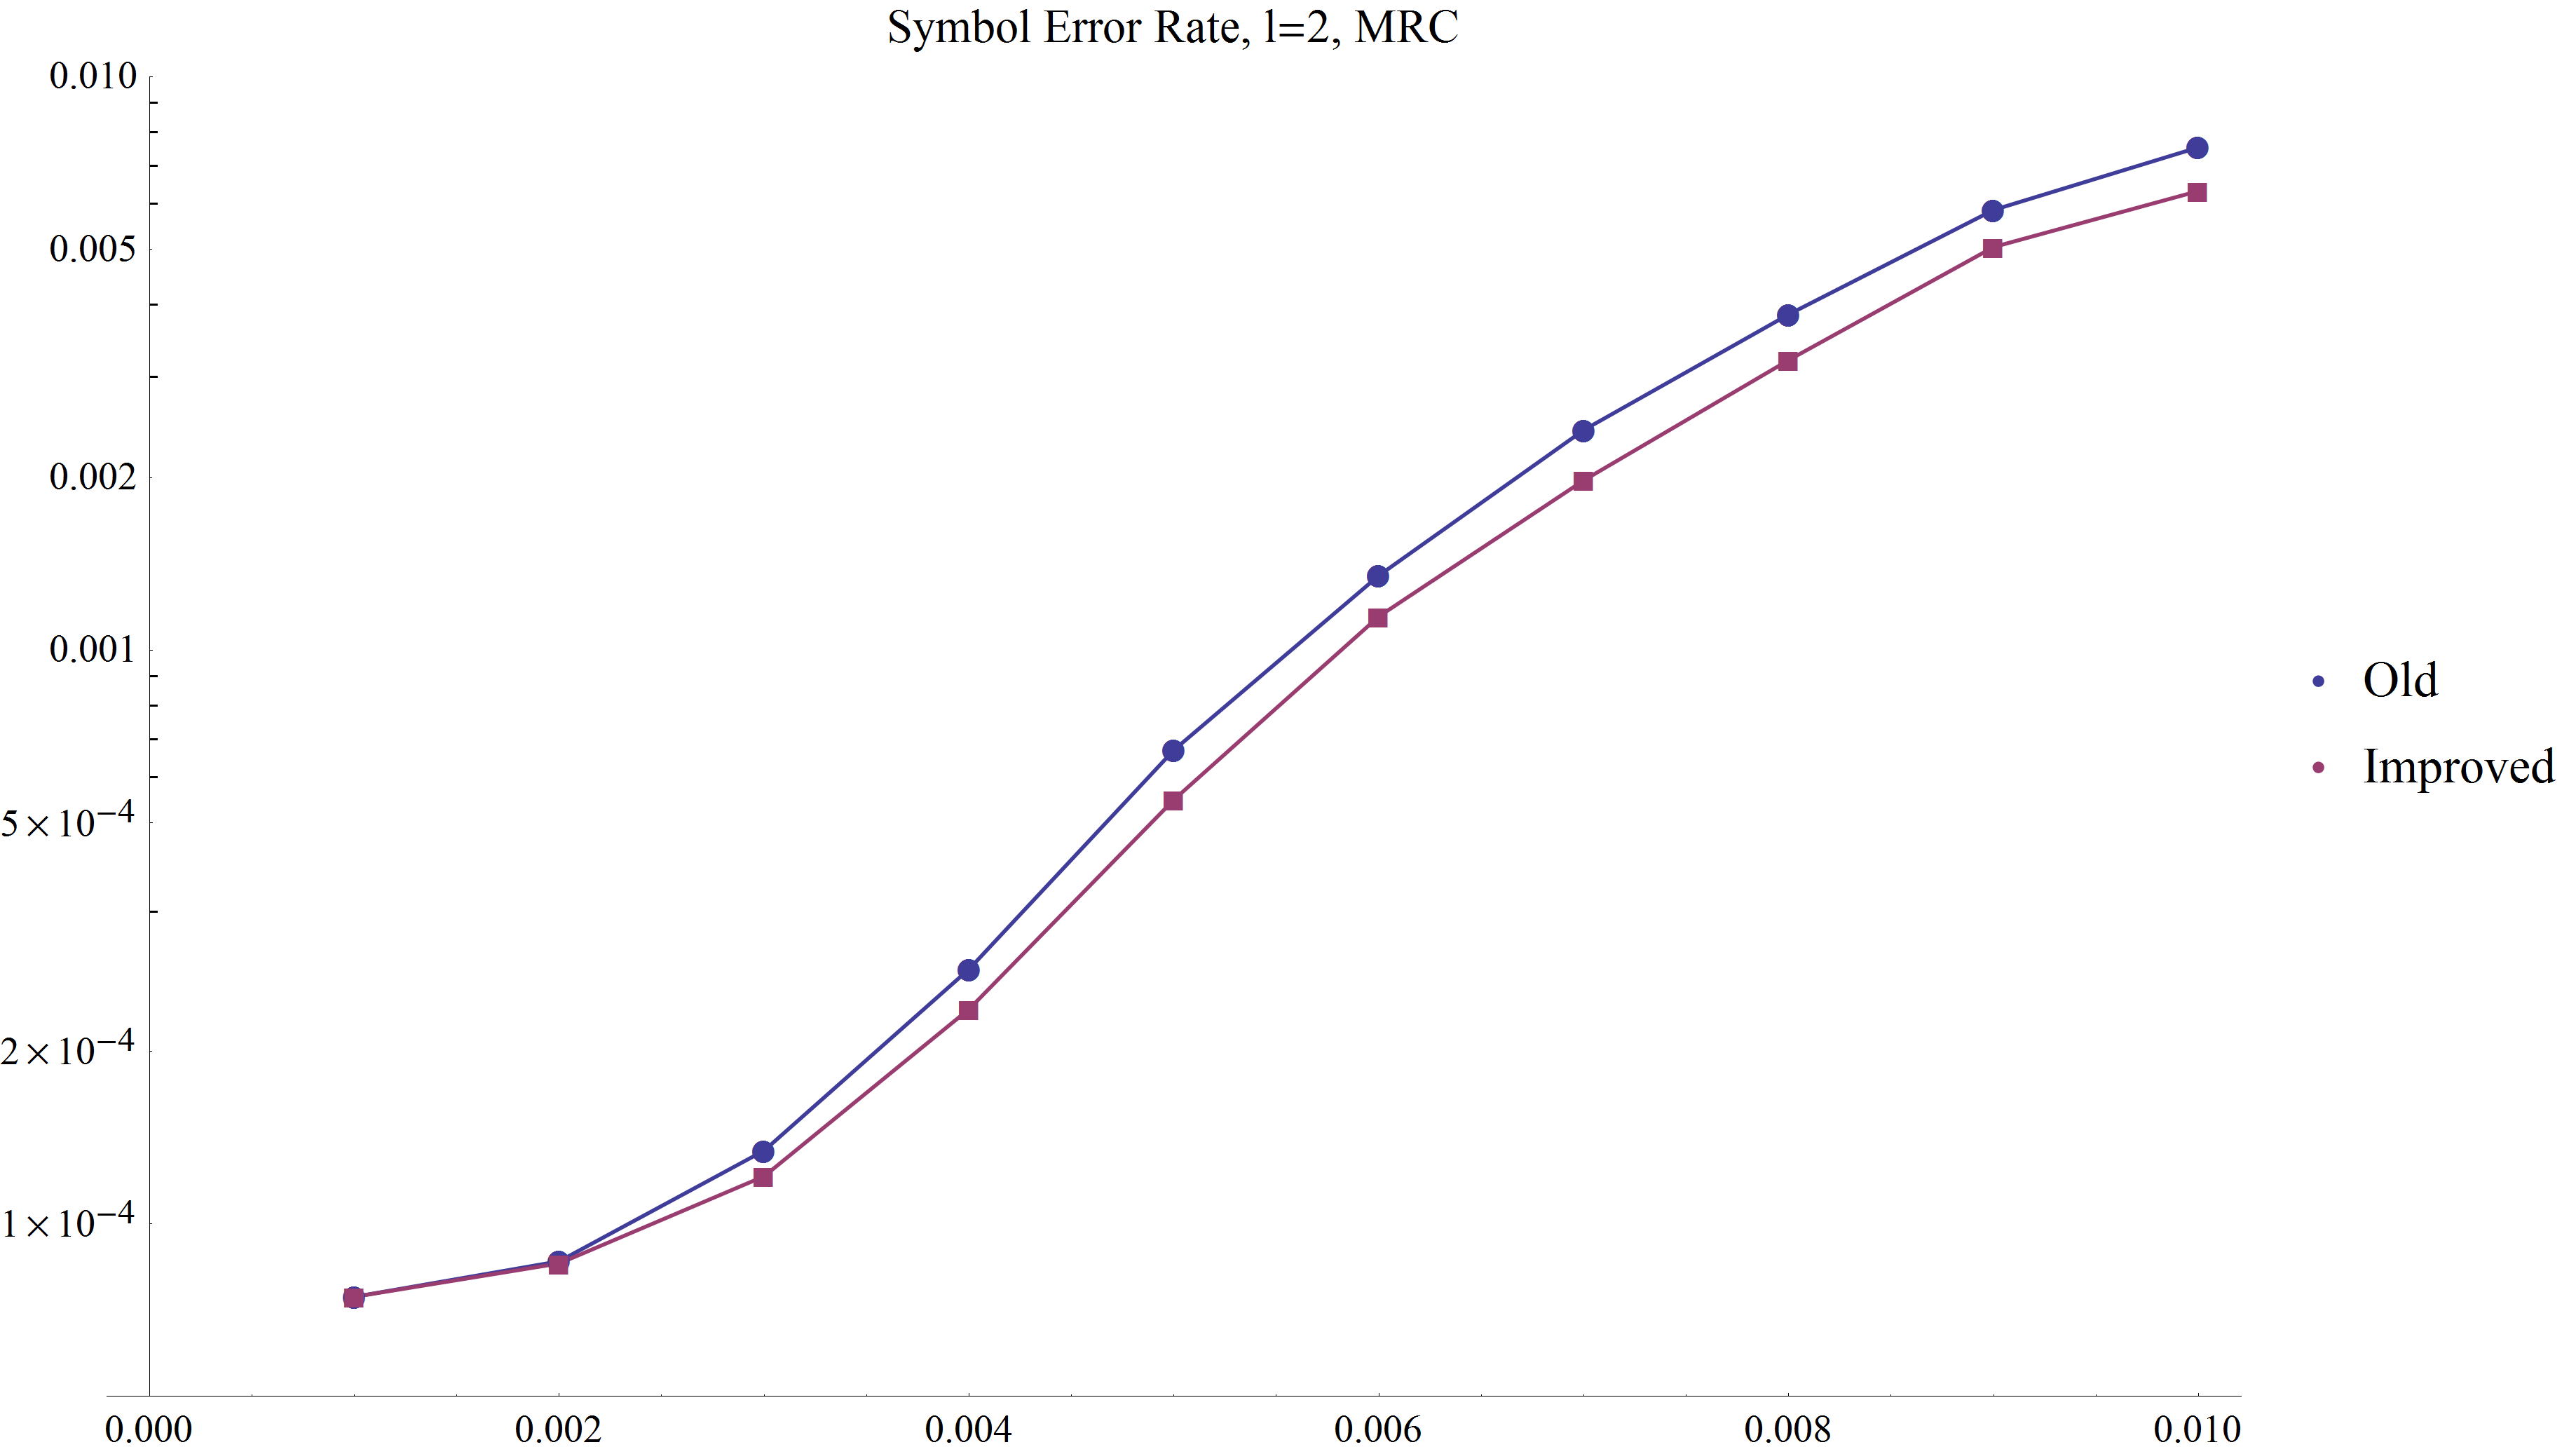
\includegraphics[width=\linewidth]{../../../plots/MRC_SER.png}
\caption{Symbol Error Rate for 2-channel MRC system with
Tikhonov-distributed timing error}
\end{figure}